\section{Natural Language Toolkit - Initial Modelling}
\label{subsection:nltk-initial_modelling}

The first model was developed using the primary dataset, data that has been cleansed but stop words have not been removed, and the Python NLTK. A Naive Bayes learner using a feature based bag of words approach was chosen. The data was stored in the NLTK corpus format where each question was individually written to a file in a folder that represented whether it was classified as bullying or not bullying. For reference, this structure is shown in Figure \ref{fig:chapter5:corpus_structure}

\begin{figure}[htbp]
	\centering
	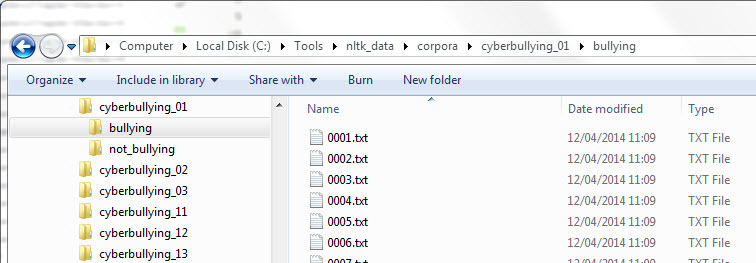
\includegraphics[width=0.85\textwidth]{Figures/Chapter5/corpus_structure.jpg}
	\caption[The structure of the primary datset corpus]{The structure of the primary dataset is shown with the top level folder containing a folder for the bullying questions and the not bullying questions. A file per question is created.}
	\label{fig:chapter5:corpus_structure}
\end{figure}

\subsection{Model Development}

The development of a NLTK classifier model is a relatively straight forward task. The first step is to create a categorised plain text corpus reader. The reader takes three parameters. The first parameter is the root folder for the corpus, the second is a regular expression used to identify the files in the corpus, the third is a regular expression used to determine the category names which are derived from the folder names within the corpus. In the code snippet shown in Listing \ref{lst:chapter5.1:snipet_01}, lines 1 to 5, the corpus to be read is \verb|cyberbullying_01| and all files with a \verb|.txt| extension are included. Now that the reader is initialised the next step is to identify the file ids of each category type.

\begin{lstlisting}[caption={Creating the categorised plain text corpus reader},label=lst:chapter5.1:snipet_01]
# Set the working folder to the nltk_data corpora folder
os.chdir ('c:/Tools/nltk_data/corpora')
reader = CategorizedPlaintextCorpusReader('./cyberbullying_01',
                                          r'.*\.txt',
                                          cat_pattern=r'(\w+)/*')
\end{lstlisting}

Identifying the file ids of each category is just a matter of calling the \verb|fileids| method passing the category name of the required file ids. The code snippet in Listing \ref{lst:chapter5.1:snipet_02} returns two file lists the first, \verb|pos_ids| is a list of all the files, including each files relative path, in the positive or bullying category while the \verb|neg_ids| is the list of all files in the negative or not bullying category. 

\begin{lstlisting}[caption={Identifying the positive and negative file ids},label=lst:chapter5.1:snipet_02]
# The questions containing bullying are the positive tests
pos_ids = reader.fileids('bullying')

# The questions not containing bullying are the negative tests
neg_ids = reader.fileids('not_bullying')
\end{lstlisting}

Figure \ref{fig:chapter5:pos_ids} is a screen capture showing the first nine files in the positive, bullying, category and that there are 1,644 files in this category. There are 7,899 files in the negative or not bullying category.

\begin{figure}[htbp]
	\centering
	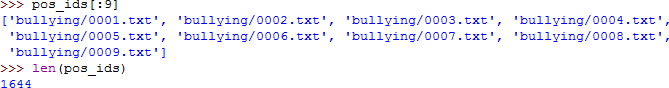
\includegraphics[width=1\textwidth]{Figures/Chapter5/pos_ids.jpg}
	\caption[List of files for the bullying category]{Screen capture showing the first nine files in the positive, bullying, category and also that there are 1,644 files in this category}
	\label{fig:chapter5:pos_ids}
\end{figure}

The NLTK uses the concept of a feature, in this case a word or token, and the Naive Bayes Classifier in the NLTK operates solely on whether a feature is present in a sample or not. The code in Listing \ref{lst:chapter5.1:snipet_03} shows how the positive and negative feature dictionaries are generated. The first three positive features are shown in Figure \ref{fig:chapter5:pos_feat} with the second sample highlighted to help distinguish each sample. Examining this second sample further, it can be seen that it is a Python dictionary containing fourteen words where each value has been given a value of true to signify their presence in the sample. Each sample is also categorised as bullying. It should be noted that all sentence word order has been lost as would be expected when using a bag of words approach. A similar process is performed to created the negative features. 

\begin{lstlisting}[caption={Generation of the positive and negative feature dictionaries},label=lst:chapter5.1:snipet_03]
def word_feats(words):
    return dict([(word, True) for word in words])

pos_feat = [(word_feats(reader.words(fileids=[f])),
             'bullying')
            for f in pos_ids]

neg_feat = [(word_feats(reader.words(fileids=[f])),
             'not_bullying')
            for f in neg_ids]
\end{lstlisting}

\begin{figure}[htbp]
	\centering
	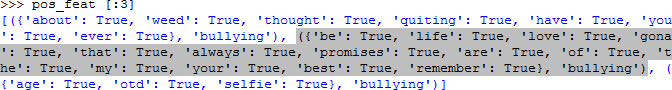
\includegraphics[width=1\textwidth]{Figures/Chapter5/pos_feat.jpg}
	\caption[Sample positive features]{Screen capture showing the first three positive features}
	\label{fig:chapter5:pos_feat}
\end{figure}

Next, the Naive Bayes learner is trained and it's performance calculated. Unfortunately, NLTK does not natively support cross validation. This meant that ten-fold cross validation had to be manually implemented in code. Full details of the implementation of the cross validation can be seen in Appendix \ref{app:simple_nltk}. Using a simple cross validation solution, the positive and negative samples were divided into ten parts. Nine of the positive and negative parts were joined together to create the training dataset and the remaining positive and negative parts joined to create the test dataset. A Naive Bayes classifier was then created using the training dataset as shown in Listing \ref{lst:chapter5.1:snipet_04}. Also shown, lines 4 - 8, is the generation of a reference set and test set to be used to calculate the performance of the classifier. To achieve this the actual classification of each of the test samples is loaded into the reference set and the value for the sample returned from the classifier is loaded into the test set. Then, using the NLTK metrics package, the performance of the classifier is calculated. For example, line 12 shows the calculation of the precision for the positive bullying samples. Finally line 18 will display the top 5 most informative features of the classifier.

\begin{lstlisting}[caption={Generation of the positive and negative feature dictionaries},label=lst:chapter5.1:snipet_04]
# Create the classifier using the train dataset
classifier = NaiveBayesClassifier.train(train)
 
#Populate the metrics sets with values
for i, (feats, label) in enumerate(test):
    refsets[label].add(i)
    observed = classifier.classify(feats)
    testsets[observed].add(i)
        
# Calculate precision. recall, f-measure
#   and accuracy
pos_pre  += nltk.metrics.precision(refsets['bullying'],
                                   testsets['bullying'])
...
# Show the top 5 most informative features
classifier.show_most_informative_features(5)
\end{lstlisting}

Once the cross validation testing has been completed then the average performance measures are calculated. A simplified visual representation of the process used to develop the first model using the NLTK is shown in Figure \ref{fig:chapter5:nltk_process_01}

\begin{figure}[htbp]
	\centering
	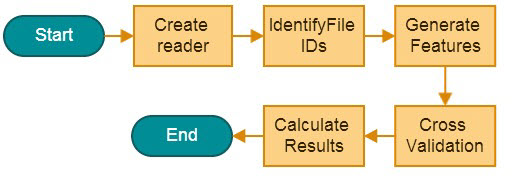
\includegraphics[width=0.85\textwidth]{Figures/Chapter5/nltk_process_01.jpg}
	\caption[NLTK model development process]{Simplified visual representation of the process used to develop the first model using the NLTK}
	\label{fig:chapter5:nltk_process_01}
\end{figure}

\subsection{Model Execution and Performance}

The NLTK Naive Bayes classifier described is then run on the primary dataset. The performance results and top five most informative features of the tenth cross validation run are shown in the screen capture in Figure \ref{fig:nltk_process_results_01}

\begin{figure}[htbp]
	\centering
	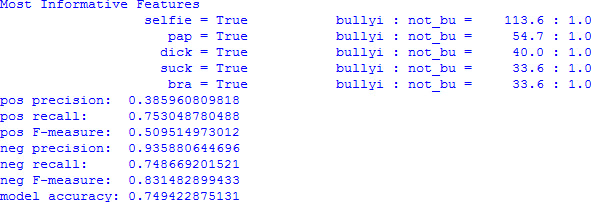
\includegraphics[width=.85\textwidth]{Figures/Chapter5/nltk_process_results_01.jpg}
	\caption[Performance measurements for initial NLTK classifier]{Screen capture of the top five most informative features from the tenth cross validation run and also the overall performance measurements for the NLTK classifier}
	\label{fig:nltk_process_results_01}
\end{figure}

Considering the top five most informative features, it is clear that these tokens, real words in this example, could easily be included in a question that was bullying in nature. The overall average accuracy of the model, just under 75\%, could suggest that this was a very successful first attempt at developing a model to predict bullying. However, looking closely at the precision and the recall for the different classes this is clearly not the case. The negative class precision, 93.6\%,  shows that nearly every sample classified as not bullying was an actual not bullying sample. Add to this a negative class recall value of 74.8\% and the model correctly identified nearly three out of every four not bullying questions. Examining the positive class next a recall value is seen which, at 75.3\%, shows that three-quarters of all bullying questions were correctly identified. However, a precision value of just 38.6\% shows that only two out of every five samples classified as bullying were  bullying questions implying that three out of every five samples classified as bullying were, in fact, not bullying questions. 

The model developed was then run on all seven datasets. The performance results for each dataset are shown in Figure \ref{fig:nltk_process_chart_01}.

\begin{figure}[htbp]
	\centering
	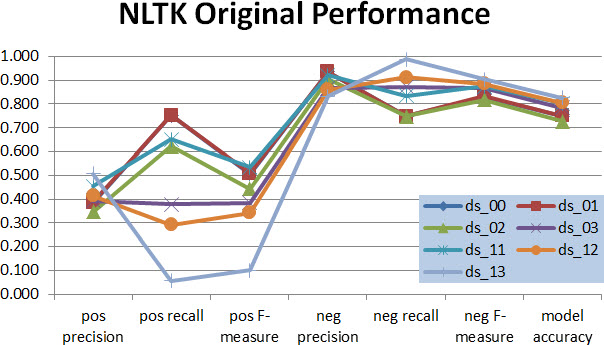
\includegraphics[width=.75\textwidth]{Figures/Chapter5/nltk_process_chart_01.jpg}
	\caption[Initial NLTK model performance across datasets]{Graph showing the performance of the initial NLTK Naive Bayes model across the seven manually crafted datasets}
	\label{fig:nltk_process_chart_01}
\end{figure}

\subsection{Model Analysis}
The first observation from an analysis of the data is that the precision of the model in predicting the positive class, the bullying questions, is poor when compared to the values obtained for the negative class with an average value of 41\% compared to an average value of 89\%. Although the average performance for recall for the positive class is 50\% this figure is not representative because of the value achieved for \verb|ds_13|, tri-grams with stop words removed, which is less than 10\%. 

Taking all performance measures into account, it could be said that the best performance achieved by this model was with \verb|ds_11|, uni-grams with stop words removed. However, with a precision value for the positive class of 45.3\% and a recall value of 65.2\% the results are far from satisfactory. This was just an initial modelling attempt and there are many changes that could be made to this model to improve its performance. Addressing class imbalance, only selecting the features that have the highest impact and by changing from the feature based approach offered by NLTK to the more statistical TF-IDF implementation offered by the Scikit-Learn package are some of the options to consider. It should also be noted that the Scikit-Learn package comes with its own cross validation implementation which will lead to a simplification of the code used.

\subsection{Further Exploration}

Before leaving this first simple model it was decided to determine if there was any advantage gained, or different results achieved, by generating the bi-grams and tri-grams up front. To test this, a simple change was needed to the \verb|word_feats| function to return bi-grams or tri-grams. Returning bi-grams is shown in Listing \ref{lst:chapter5.1:snipet_05}. Four new models were created using the bi-grams and tri-grams datasets generated from \verb|dataset_01| and \verb|dataset_11|.

\begin{lstlisting}[caption={Generation of the positive and negative feature dictionaries},label=lst:chapter5.1:snipet_05]
from nltk import bigrams
from nltk import trigrams
...
def word_feats(words):
    return dict([(word, True) for word in bigrams(words)])
\end{lstlisting}

The results generated by these new models were then compared to the original models where the bi-gram and tri-gram tokens were manually created beforehand. The different models were compared in three areas. The first, and easiest to compare, was average execution time. The average run time for each model was determined and it was found that generating the bi-grams or tri-grams during model execution did add to the overall execution time as can be seen in Table \ref{tab:chapter5:ngram_generation}. With a maximum time of 0.1 seconds to generate all tri-grams in advance, the longest to create, it is clear that there is a time advantage to creating all n-grams upfront. In Table \ref{tab:chapter5:ngram_generation} the first column is the model execution where the n-grams were generated before hand. Thee second column is the time for n-grams created during model execution. Column three is the time difference in seconds and the fourth column is the percentage increase in time.

\begin{table}[h]
\centering
\caption[N-gram generation increases execution time]{Table showing average model execution time increase when n-grams are generated as part of the modelling process}
\label{tab:chapter5:ngram_generation}
\begin{tabular}{rrrrr}
	\toprule
     & \textbf{orig}  & \textbf{new} & \textbf{diff} & \textbf{percent}    \\
    \midrule
    bi-gram & 19.399 & 20.549 & 1.150 & 5.9\%  \\
    tri-gram & 23.116 & 24.647 & 1.531 & 6.6\%  \\
    bi-gram ns & 14.357 & 15.685 & 1.328 & 9.3\%   \\
    tri-gram ns & 11.477 & 14.225 & 2.748 & 23.9\%   \\
    \bottomrule
    \end{tabular}
\end{table}

The second comparison is the performance of the models. The results of this analysis is shown in Figure \ref{fig:nltk_process_chart_02}. A cursory look at these charts  shows that the generation of the n-grams during the model execution did not improve the overall performance of the model. It may, it fact, have had a slightly negative impact which can be seen in the positive class recall and f-measure values. In all charts the top line in the legend represents the performance of the original model. For example, in the chart labelled ``Bi-grams no stop words'', the \verb|01_12| series, represented by the blue line shows, the performance values of the original model, \verb|01|, using bi-grams generated from the dataset where stop words have already been removed, \verb|_12|. The orange line, \verb|02_12|, is from the second model where bi-grams were generated during model execution.

\begin{figure}[htbp]
	\centering
	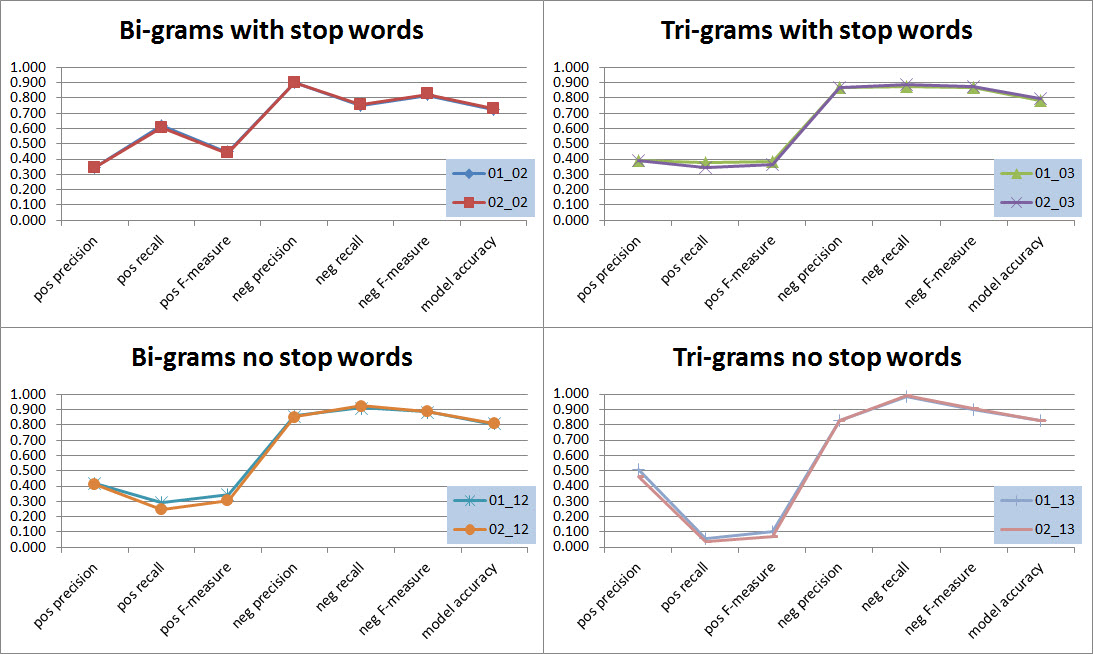
\includegraphics[width=1\textwidth]{Figures/Chapter5/nltk_process_chart_02.jpg}
	\caption[Comparison of pre-generated and in model n-gram generation]{Graphs showing a comparison or model performance when n-grams are pre-generated or generated during model execution}
	\label{fig:nltk_process_chart_02}
\end{figure}

The final analysis performed was a comparison of the most informative features returned during each model execution. Ten-fold cross validation was used and the top five most informative features were returned. The results of the number of most informative features comparison is summarised in Table \ref{tab:chapter5:informative_features}.

Whilst initially it appeared that there were a number of significant differences, after an investigation it was found that sometimes the most informative features with the same ratio values were sorted differently between the two model types. The other cause of the differences was the way the datasets were processed when the n-grams were generated during execution. When the tri-grams were generated up front, samples that had only two words never got included in the datasets submitted to the modelling process. This meant that there were only 1,049 positive and 4,915 negative samples for tri-grams with no stop words. However, there are 1,637 and 7,800 samples respectively in the uni-grams with no stop words dataset. As the ten-fold cross validation datasets were created before the n-grams were generated, this lead to a different split of the samples in the two models being compared. 

\begin{table}[h]
\centering
\caption[Most informative feature comparison]{Table showing the number of the most informative features that were different when n-grams were generated during model execution using the NLTK compared to being generated beforehand}
\label{tab:chapter5:informative_features}
\begin{tabular}{rc}
	\toprule
    \textbf{Model} & \textbf{Number} \\
    \textbf{Type} & \textbf{Differences} \\
    \midrule
    Bi-grams & 5 \\
    Tri-grams & 2   \\
    Bi-grams no stop words & 3    \\
    Tri-grams no stop words & 15    \\
    \bottomrule
    \end{tabular}
\end{table}

Based on the analysis given it was decided that for the simple NLTK model developed here it did not matter that the n-gram datasets were generated beforehand. It should be noted, however, that the models generated used all the classified data available and they were not tested on unseen data. This is not considered an issue as the performance results achieved here will be considered as a baseline against which all subsequent models could be compared.